\documentclass{ximera}

\graphicspath{{./}{eulerCharacteristic}}


\title{Drug Decay}
\author{Bart Snapp \and Brad Findell}
\begin{document}
\begin{abstract}
Here we investigate various models for the decay of drugs in our bodies.  
\end{abstract}
\maketitle

\begin{question}
A solution to a algebraic equation is usually a $\answer[format=string]{number}$ that makes the equation true.  A solution to a differential equation is a $\answer[format=string]{function}$ that makes the equation true.  
\end{question}

Pharmacokinetics is the study of the behavior of drugs and other substances administered to living organisms.  
The well-established general model for 
the elimination of a given drug from the body of a given human being is given by the differential equation 
$$y'(t)=-\frac{ky(t)}{A+y(t)}$$
where $y(0)$ is the initial concentration in, say, milligrams per liter, and $y(t)$ is the concentration at time $t$.  The constants $k$ and $A$ depend, of course, on the particular drug and the particular human being. 


\begin{question}
When the drug in question is alcohol, $y(t)$ is usually rather large in comparison to $A$.   With this assumption, we can approximate the general model with a simpler model, $y'(t)=\answer{-k}$.    

If where $C=y(0)$ the initial concentration at time $t=0$, then the general solution to this differential equation is 
\[  
y(t) =\answer{ -kt + C}.  
\]

What kind of function is this? $\answer[format=string]{linear}$

And the second derivative of this function is \wordChoice{\choice{positive}\choice{negative}\choice[correct]{zero}\choice{unknown}}.  
\end{question}

\begin{question}
When the drug is alcohol, which of the following graphs shows the best solution for the simpler model, $y'(t)=-k$, with $y(0)=4$?
\begin{multipleChoice}
\choice{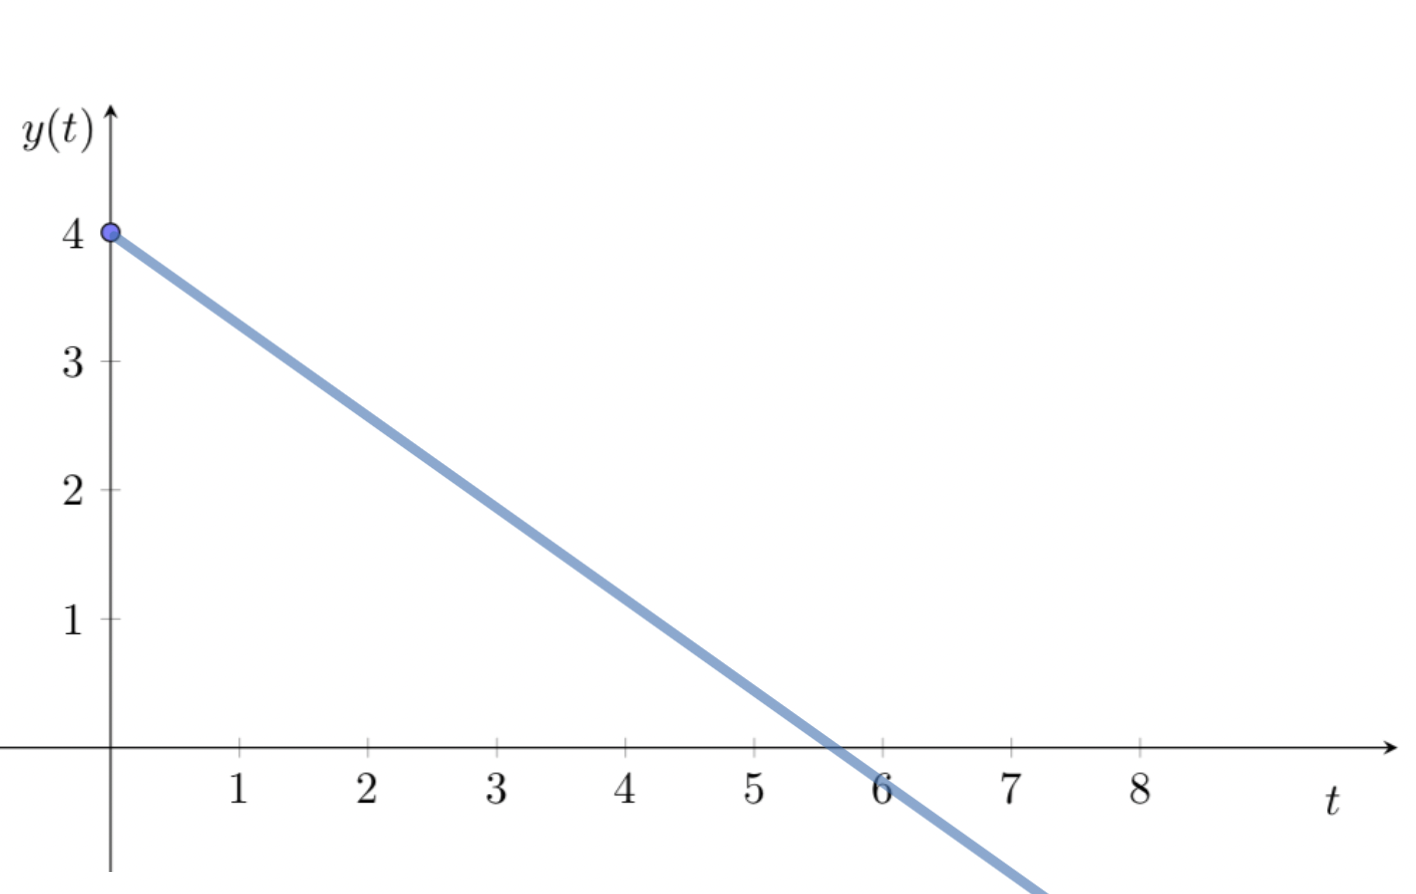
\includegraphics{graph5.png}}
\choice{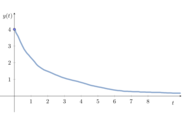
\includegraphics{graph2.png}}
\choice{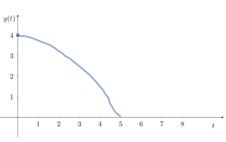
\includegraphics{graph3.png}}
\choice[correct]{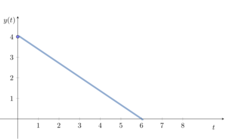
\includegraphics{graph4.png}}
\choice{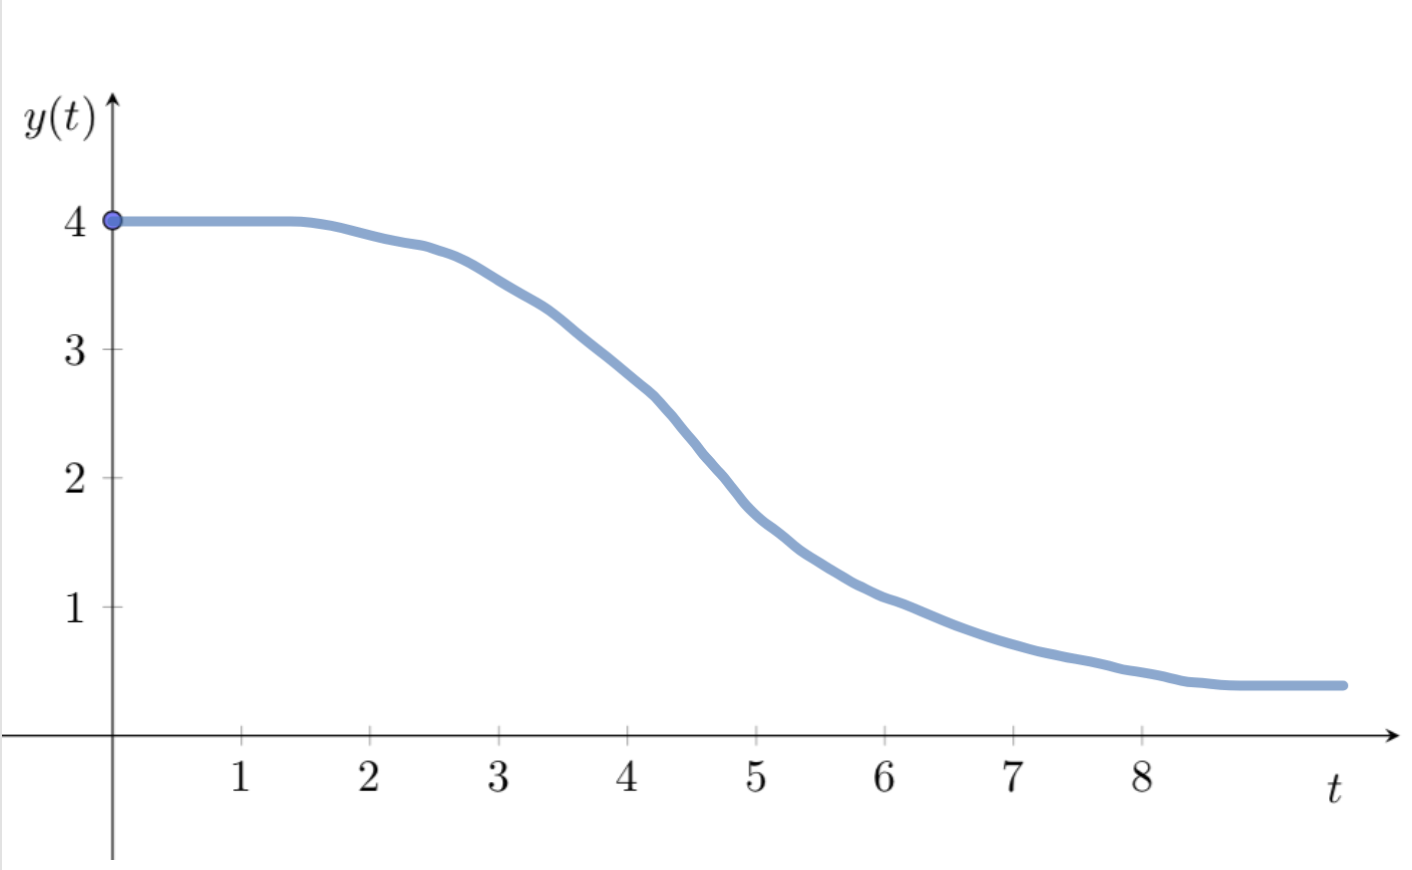
\includegraphics{graph6.png}}
\choice{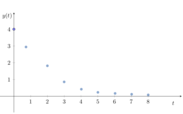
\includegraphics{graph7.png}}
\end{multipleChoice}

\begin{question}
Correct.  The reasons for my choice:  
\begin{selectAll}
\choice{Should be concave up}
\choice{Should be concave down}
\choice[correct]{Should have zero concavity}
\choice{Should be always increasing}
\choice[correct]{Should be always decreasing}
\choice{Should be constant}
\choice{Should be sometimes increasing, sometimes decreasing}
\end{selectAll}

More reasons for my choice: 
\begin{selectAll}
\choice[correct]{Should be linear}
\choice{Should be exponential decay}
\choice{Should be exponential growth}
\choice[correct]{$y(t)$ should never be negative}
\choice{Should be discrete}
\choice[correct]{Should be continuous}
\end{selectAll}
\end{question}
\end{question}


Agan, the general model for  the elimination of a given drug from the body of a given human being is given by the differential equation 
$$y'(t)=-\frac{ky(t)}{A+y(t)}$$
where $y(0)$ is the initial concentration in, say, milligrams per liter, and $y(t)$ is the concentration at time $t$. 

\begin{question}
When the drug in question is cocaine, $y(t)$ is usually very small in comparison to $A$.   With this assumption, we can approximate the general model with a simpler model, $y'(t)=\answer{-\frac{k}{A}}y(t)$.    

If where $C=y(0)$ the initial concentration at time $t=0$, then the general solution to this differential equation is 
\[  
y(t) =\answer{Ce^{-\frac{k}{A}t}}. 
\]

What kind of function is this? $\answer[format=string]{exponential}$

And the second derivative of this function is \wordChoice{\choice[correct]{positive}\choice{negative}\choice{zero}\choice{unknown}}.  
\end{question}

\begin{question}
When the drug is alcohol, which of the following graphs shows the best solution for the simpler model, $y'(t)=-k$, with $y(0)=4$?
\begin{multipleChoice}
\choice{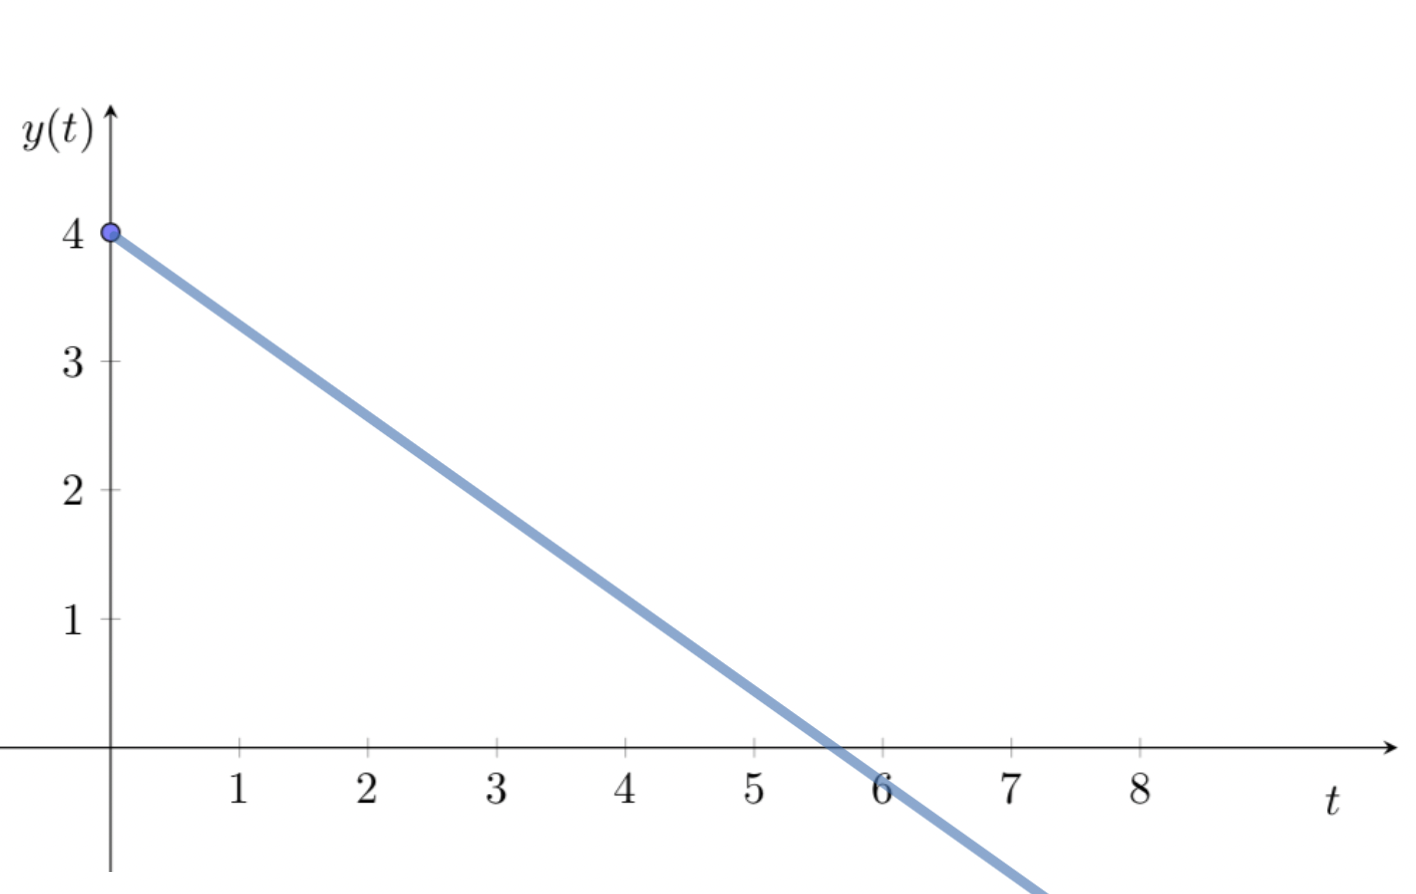
\includegraphics{graph5.png}}
\choice[correct]{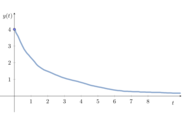
\includegraphics{graph2.png}}
\choice{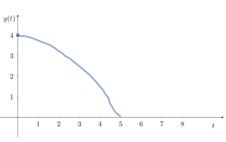
\includegraphics{graph3.png}}
\choice{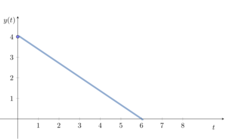
\includegraphics{graph4.png}}
\choice{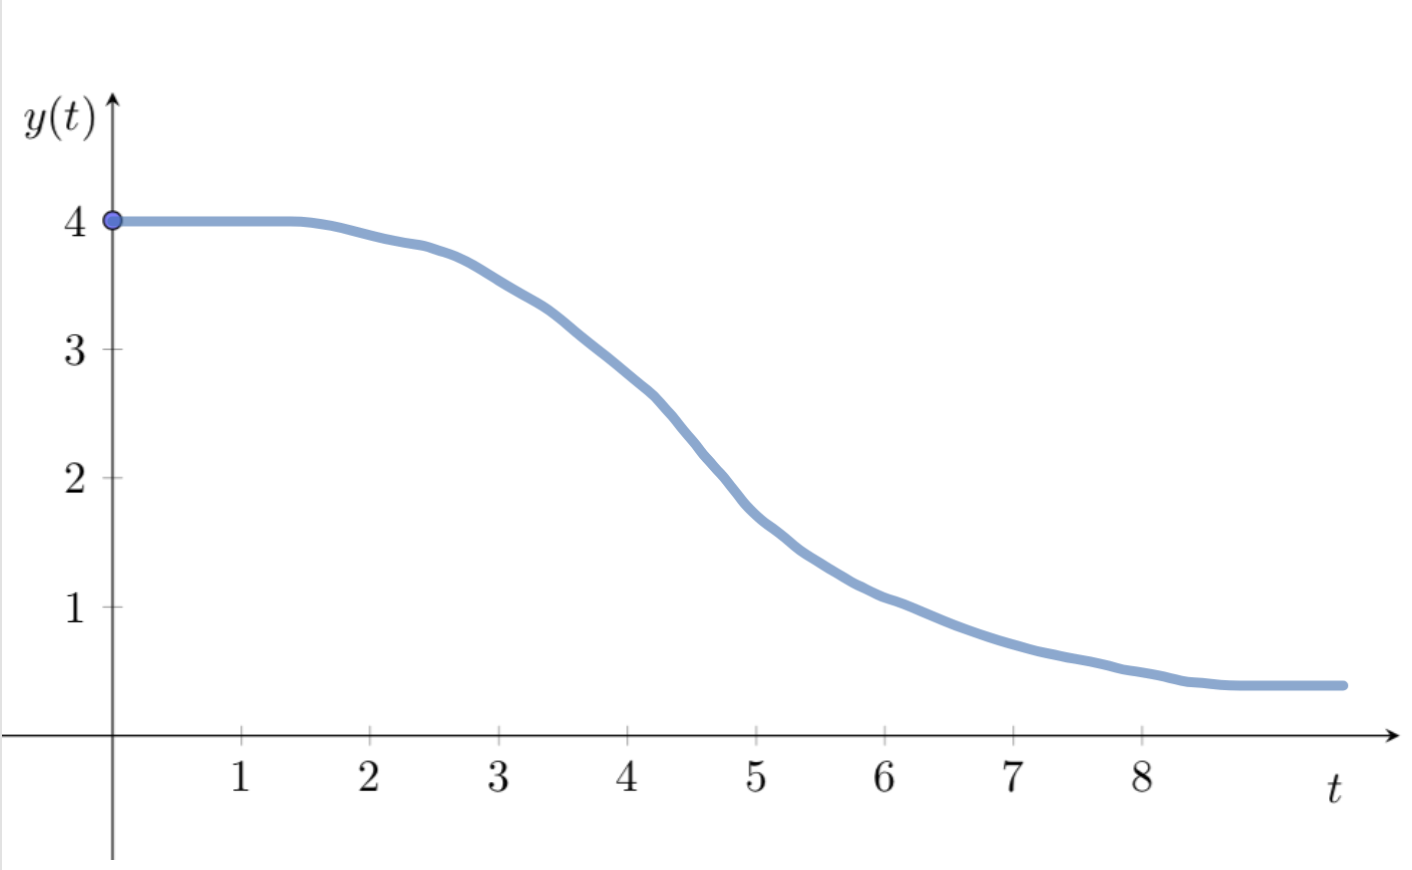
\includegraphics{graph6.png}}
\choice{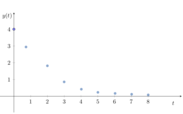
\includegraphics{graph7.png}}
\end{multipleChoice}

\begin{question}
Correct.  The reasons for my choice:  
\begin{selectAll}
\choice[correct]{Should be concave up}
\choice{Should be concave down}
\choice{Should have zero concavity}
\choice{Should be always increasing}
\choice[correct]{Should be always decreasing}
\choice{Should be constant}
\choice{Should be sometimes increasing, sometimes decreasing}
\end{selectAll}

More reasons for my choice: 
\begin{selectAll}
\choice{Should be linear}
\choice[correct]{Should be exponential decay}
\choice{Should be exponential growth}
\choice[correct]{$y(t)$ should never be negative}
\choice{Should be discrete}
\choice[correct]{Should be continuous}
\end{selectAll}
\end{question}
\end{question}


\end{document}
